\subsection{02-26-2-ThanhHoa-SoGD-L1}
\caulc
\Opensolutionfile{ans}[ans/02-26-2-ThanhHoa-SoGD-L1-P1]
%%---Câu 1---%%
\begin{ex}%[1D1N5-3]
	Họ nghiệm của phương trình $\cos x=1$ là
	\choice
	{$x=\dfrac{k\pi}{2}, k \in \mathbb{Z}$}
	{$x=k\pi, k \in \mathbb{Z}$}
	{$x=\dfrac{\pi}{2} + k2\pi, k \in \mathbb{Z}$}
	{\True $x = k2\pi, k \in \mathbb{Z}$}
	\loigiai{
	Ta có $\cos x = 1 \Leftrightarrow x = k2\pi, k \in \mathbb{Z}$.
	}
\end{ex}
%%---Câu 2---%%
\begin{ex}%[1D2N3-4]
	Cho cấp số nhân $\left( u_n \right)$ với $u_1 = 2$ và công bội $q = 3$. Số hạng thứ $4$ của cấp số nhân bằng
	\choice
	{$24$}
	{\True $54$}
	{$162$}
	{$48$}
	\loigiai{
	Có $u_4 = u_1 \cdot q^3 = 2 \cdot 3^3 = 54$.
	}
\end{ex}
%%---Câu 3---%%
\begin{ex}%[1D6N4-2]
	Tập nghiệm của phương trình $\log_3(2x - 1) = \log_3(x - 1)$ là
	\choice
	{\True $S = \varnothing$}
	{$S = \{0\}$}
	{$S = \{-2\}$}
	{$S = \{2\}$}
	\loigiai{
	Điều kiện: $x > 1$.\\
	Phương trình tương đương $2x - 1 = x - 1 \Leftrightarrow x = 0$.\\
	So với điều kiện ta được tập nghiệm $S = \varnothing$.
	}
\end{ex}
%%---Câu 4---%%
\begin{ex}%[1H4N4-2]
	\immini{Cho hình hộp $ABCD.A'B'C'D'$. Xét các mệnh đề sau:
	\begin{enumerate}[i)]
	\item $AB \parallel CD$; 
	\item $BB' \parallel (CC'D'D)$; 
	\item $(A'B'C') \parallel (ABD)$.
	\end{enumerate}
	Số mệnh đề đúng trong các mệnh đề trên là
	\choice
	{$1$}
	{$2$}
	{\True $3$}
	{$0$}
	}{\begin{tikzpicture}[scale=1, font=\footnotesize, line join=round, line cap=round, >=stealth]
	\def\bc{4} % cạnh BC
	\def\ba{2} % cạnh BA
	\def\gocB{35} % góc B của đáy
	\coordinate[label=below left:$B$] (B) at (0,0);
	\coordinate[label=above left:$A$] (A) at (\gocB:\ba);
	\coordinate[label=below:$C$] (C) at (\bc,0);
	\coordinate[label=right:$D$] (D) at ($(C)-(B)+(A)$);
	\coordinate[label=above left:$A'$] (A') at ($(A)+(90:\bc)$);
	\coordinate[label=left:$B'$] (B') at ($(B)-(A)+(A')$);
	\coordinate[label=below right:$C'$] (C') at ($(C)-(A)+(A')$);
	\coordinate[label=right:$D'$] (D') at ($(D)-(A)+(A')$);
	\draw (B')--(B)--(C)--(D)--(D')--(A')--(B')--(C')--(D') (C)--(C');
	\draw[dashed] (A')--(A)--(D) (A)--(B);
	\foreach \diem in {A,B,C,D,A',B',C',D'}	\fill (\diem)circle(1.5pt);
	\end{tikzpicture}
	}
	\loigiai{
	Do $ABCD$ là hình bình hành nên $AB \parallel CD$, suy ra $i)$ đúng. \\
	Do $ABCD.A'B'C'D'$ là hình hộp nên $BB' \parallel CC'$, suy ra $BB' \parallel (CC'D'D)$. Vậy $ii)$ đúng. \\
	Do $ABCD.A'B'C'D'$ là hình hộp nên $(A'B'C'D') \parallel (ABCD)$, suy ra $iii)$ đúng. \\
	Kết luận: Cả ba mệnh đề trên đều đúng.
	}
\end{ex}
%%---Câu 5---%%
\begin{ex}%[1H8N7-2]
	Cho khối chóp tam giác $S.ABC$ có chiều cao bằng $3$, đáy là tam giác $ABC$ có diện tích bằng $10$. Thể tích khối chóp $S.ABC$ bằng
	\choice
	{$2$}
	{$15$}
	{\True $10$}
	{$30$}
	\loigiai{
	Thể tích khối chóp $S.ABC$ là $V = \dfrac{1}{3} \cdot B \cdot h = \dfrac{1}{3} \cdot 10 \cdot 3 = 10$.
	}
\end{ex}
%%---Câu 6---%%
\begin{ex}%[2D1N5-1]
	\immini{Cho hàm số bậc ba $y = ax^3 + bx^2 + cx + d$ ($a, b, c, d \in \mathbb{R}$) có đồ thị như hình bên. Mệnh đề nào dưới đây đúng?
	\choice
	{$a>0$, $d > 0$}
	{\True $a<0$, $d > 0$}
	{$a>0$, $d < 0$}
	{$a<0$, $d < 0$}
	}{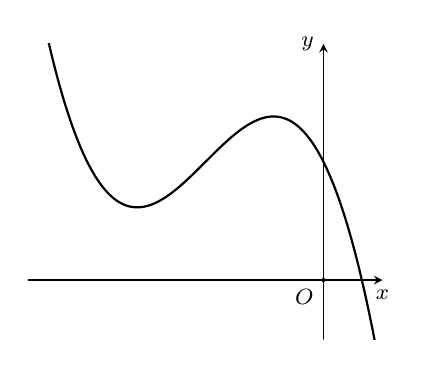
\begin{tikzpicture}[scale=.75, font=\footnotesize, line join=round, line cap=round, >=stealth]
	\def\a{-1/4} \def\b{-3/2}\def\c{-2}\def\d{2}
	\draw[->] (-5,0) -- (1,0) node[below] {$x$};
	\draw[->] (0,-1) -- (0,4) node[left] {$y$};
	\fill (0,0) circle (1pt) node[below left]{$O$};
	\clip (-5,-1)rectangle(1,4);
	\draw[thick,samples=150,smooth,domain=-5:5] plot(\x,{\a*(\x)^3+(\b)*(\x)^2+(\c)*\x+(\d)});
	\end{tikzpicture}}
	\loigiai{
	Ta có: $\lim_{x \to +\infty} y = -\infty \Rightarrow$ đồ thị nhánh ngoài cùng của hàm số hướng đi xuống nên hệ số $a < 0$. \\
	Giao điểm của đồ thị hàm số với trục tung $Oy: x = 0$ là điểm nằm bên trên trục hoành nên khi $x = 0 \Rightarrow y = d > 0$.
	}
\end{ex}
%%---Câu 7---%%
\begin{ex}%[2H2N1-1]
	\immini{Cho lăng trụ đứng $ABC.A'B'C'$. Đáy là tam giác $ABC$ vuông cân tại $B$ (Hình minh họa bên). Khi đó góc giữa vectơ $\overrightarrow{AB}$ và vectơ $\overrightarrow{A'C'}$ bằng bao nhiêu?
	\choice
	{\True $45^{\circ}$}
	{$60^{\circ}$}
	{$90^{\circ}$}
	{$135^{\circ}$}
	}{\begin{tikzpicture}[scale=1, font=\footnotesize, line join=round, line cap=round, >=stealth]
	\def\ac{4} % cạnh AC
	\def\ab{2} % cạnh AB
	\def\h{3} % chiều cao
	\def\gocA{50} % góc A của đáy
	\coordinate[label=left:$A$] (A) at (0,0);
	\coordinate[label=right:$C$] (C) at (\ac,0);
	\coordinate[label=below left:$B$] (B) at (-\gocA:\ab);
	\coordinate[label=left:$A'$] (A') at ($(A)+(90:\h)$);
	\coordinate[label=below left:$B'$] (B') at ($(B)-(A)+(A')$);
	\coordinate[label=right:$C'$] (C') at ($(C)-(A)+(A')$);
	\draw (A')--(A)--(B)--(C)--(C')--(A')--(B')--(C') (B)--(B');
	\draw[dashed] (A)--(C);
	\path pic[angle radius=3mm,draw=blue] {right angle = C--B--A};
	\foreach \diem in {A,B,C,A',B',C'} \fill (\diem)circle(1.5pt);
	\end{tikzpicture}
	}
	\loigiai{
	Ta có $\overrightarrow{A'C'} = \overrightarrow{AC}$. \\
	Do đó $\left(\overrightarrow{AB}, \overrightarrow{A'C'}\right) = \left(\overrightarrow{AB}, \overrightarrow{AC}\right)= \widehat{BAC}$. \\
	Mà tam giác $ABC$ vuông cân tại $B$ nên $\widehat{BAC} = 45^{\circ} \Rightarrow \left(\overrightarrow{AB}; \overrightarrow{A'C'}\right) = 45^{\circ}$.
	}
\end{ex}
%%---Câu 8---%%
\begin{ex}%[2H2N1-1]
	Trong không gian $Oxyz$, cho điểm $A\left(2;-3;5\right)$. Gọi điểm $H$ là hình chiếu vuông góc của điểm $A$ trên mặt phẳng $\left(Oxy\right)$. Tọa độ của điểm $H$ là
	\choice
	{$H\left(0;0;5\right)$}
	{$H\left(0;-3;5\right)$}
	{$H\left(2;0;5\right)$}
	{\True $H\left(2;-3;0\right)$}
	\loigiai{
	Do $H$ là hình chiếu vuông góc của $A\left(2;-3;5\right)$ lên mặt phẳng $\left(Oxy\right)$.\\
	Suy ra $H\left(2;-3;0\right)$.
	}
\end{ex}
%%---Câu 9---%%
\begin{ex}%[2H5N1-3]
	Trong không gian $Oxyz$, cho hai điểm $A\left(0;1;1\right)$ và $B\left(1;2;3\right)$. Phương trình mặt phẳng $\left(P\right)$ đi qua điểm $A$ và có vectơ pháp tuyến $\overrightarrow{AB}$ là
	\choice
	{\True $\left(P\right)\colon x+y+2z-3=0$}
	{$\left(P\right)\colon x+y+2z-9=0$}
	{$\left(P\right)\colon x+3y+4z-7=0$}
	{$\left(P\right)\colon x+3y+4z-26=0$}
	\loigiai{
	Ta có $\left(P\right):\heva{&\text{Đi qua } A\left(0;1;1\right) \\& \text{Có vectơ pháp tuyến}\, \vec{n}_{\left(P\right)} = \overrightarrow{AB} = \left(1;1;2\right).}$ \\
	$\Rightarrow \left(P\right): 1\left(x-0\right)+1\left(y-1\right)+2\left(z-1\right)=0 \Leftrightarrow \left(P\right): x+y+2z-3=0$.
	}
\end{ex}
%%---Câu 10---%%
\begin{ex}%[2D4N1-1]
	Cho $\displaystyle\int 5^x\mathrm{\,d}x=F(x)+C$. Khẳng định nào dưới đây đúng?
	\choice
	{$F'(x)=5^x\ln 5$}
	{$F'(x)=5^x+C$}
	{$F'(x)=\dfrac{5^x}{\ln 5}$}
	{\True $F'(x) = 5^x$}
	\loigiai{
	Ta có $F'(x)=\left(F(x) + C\right)'=\left(\displaystyle\int 5^x\mathrm{\,d}x\right)'= 5^x$.
	}
\end{ex}
%%---Câu 11---%%
\begin{ex}%[2D4N3-1]
	\immini{Diện tích phần hình phẳng gạch chéo trong hình vẽ bên được tính theo công thức nào dưới đây?
	\choice
	{$\displaystyle\int\limits_{-1}^2(-2x+2)\mathrm{\,d}x$}
	{$\displaystyle\int\limits_{-1}^2(2x-2)\mathrm{\,d}x$}
	{\True $\displaystyle\int\limits_{-1}^2(-2x^2+2x+4)\mathrm{\,d}x$}
	{$\displaystyle\int\limits_{-1}^2(2x^2-2x-4) \mathrm{\,d}x$}
	}{\begin{tikzpicture}[line cap=round, line join=round,>=stealth,scale=.5,font=\footnotesize,
	declare function={xmin=-3; xmax=5; ymin=-3; ymax=4; h=1; v=1; a(\x)=\x;	c1(\x)=-(\x)^2+3; c2(\x)=(\x)^2-2*\x-1;}]
	\node[right] at (2.2,{c1(2.2)}) {$y=-x^2+3$};
	\node[right] at (.35,{c2(3.35)}) {$y=x^2-2x-1$};
	\clip (xmin,ymin) rectangle (xmax,ymax);
	\fill[gray!30] plot[domain=-1:2] ({\x},{c1(\x)}) -- plot[domain=2:-1] ({\x},{c2(\x)}) -- cycle;
	\draw[domain=xmin:xmax, variable=\x, samples=200, smooth, thick, name path=c1] plot ({\x},{c1(\x)});
	\draw[domain=xmin:xmax, variable=\x, samples=200, smooth, thick, name path=c2] plot ({\x},{c2(\x)});
	\draw[->] (xmin,0)--(xmax,0) node[above left] {$x$};
	\draw[->] (0,ymin)--(0,ymax) node[below left] {$y$};
	\node[above right] at (0,0) {$ O $};
	\draw[dashed]
	(-1,{c1(-1)}) -- (-1,0) node[below] {$-1$}
	(2,{c1(2)}) -- (2,0) node[above] {$2$};
	\end{tikzpicture}}
	\loigiai{
	Diện tích hình phẳng gạch chéo trong hình vẽ là \\
	$S = \displaystyle\int\limits_{-1}^{2} \left| (-x^2 + 3) - (x^2 - 2x - 1) \right| \mathrm{\,d}x = \displaystyle\int\limits_{-1}^{2} \left| -2x^2 + 2x + 4 \right| \mathrm{\,d}x = \displaystyle\int\limits_{-1}^{2} (-2x^2 + 2x + 4) \mathrm{\,d}x$.
	}
\end{ex}
%%---Câu 12---%%
\begin{ex}%[1D5H2-2]
	Thời gian truy cập Internet trong một buổi tối của một nhóm học sinh được cho trong bảng sau:
	\begin{center}
	\begin{tabular}{|l|c|c|c|c|c|}
	\hline
	Thời gian (phút) & $[9{,}5;12{,}5)$ & $[12{,}5;15{,}5)$ & $[15{,}5;18{,}5)$ & $[18{,}5;21{,}5)$ & $[21{,}5;24{,}5)$ \\ \hline
	Số học sinh & $3$ & $12$ & $15$ & $24$ & $2$ \\ \hline
	\end{tabular}
	\end{center}
	Tính trung vị của mẫu số liệu ghép nhóm này.
	\choice
	{\True $18{,}1$}
	{$18{,}5$}
	{$17{,}2$}
	{$15{,}6$}
	\loigiai{
	Cỡ mẫu là: $n = 3 + 12 + 15 + 24 + 2 = 56$. \\
	Nhóm chứa trung vị là $[15{,}5; 18{,}5)$. Ta có: 
	$M_{\mathrm{e}} = 15{,}5 + \dfrac{\dfrac{56}{2} - 15}{15} \cdot 3 = 18{,}1$.
	}
\end{ex}
\Closesolutionfile{ans}
\cauds
\Opensolutionfile{ans}[ans/02-26-2-ThanhHoa-SoGD-L1-P2]
%%---Câu 1---%%
\begin{ex}%[2D1H5-1]
	\immini{Cho hàm số $y = \dfrac{mx^2 + nx - 1}{px - 2}$ có đồ thị như hình vẽ bên.
	\choiceTF
	{\True Đường tiệm cận đứng của đồ thị là đường thẳng $x = 2$}
	{Hàm số nghịch biến trên khoảng $\left(1; 3\right)$}
	{Tâm đối xứng của đồ thị là điểm $I\left(3; 2\right)$}
	{\True Ta có $m + 2n - 3p = -4$}
	}{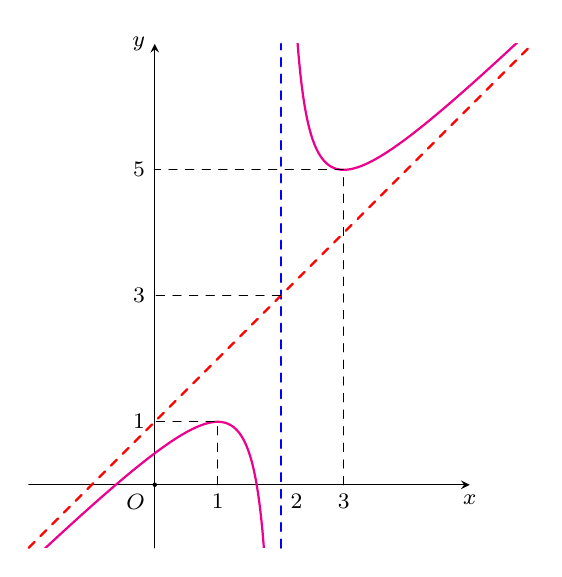
\begin{tikzpicture}[scale=.8, font=\footnotesize, line join=round, line cap=round, >=stealth]
	\def\a{1}	\def\b{-1}	\def\c{-1}	\def\d{1}	\def\e{-2}	
	\pgfmathsetmacro{\tcd}{-\e/\d}	
	\pgfmathsetmacro{\intercept}{(\b*\d - \e *\a)/\d^2}	
	\draw[->] (-2, 0) -- (5, 0) node[below] {$x$};
	\draw[->] (0, -1) -- (0, 7) node[left] {$y$};
	\fill (0, 0) circle (1pt) node[below left]{$O$};
	\draw[thick, dashed, blue] (\tcd, -1) -- (\tcd, 7);	
	\draw[thick, dashed, red] (-2, {(-2)*(\a/\d) + \intercept}) -- (6, {6*(\a/\d) + \intercept});
	\clip (-2, -1) rectangle (6, 7);
	\draw[magenta, thick, samples=150, smooth, domain=-5:{\tcd-.1}] plot (\x, {(\a*\x*\x + \b*\x + \c)/(\d*\x + \e)});
	\draw[magenta, thick, samples=150, smooth, domain={\tcd+.1}:6] plot (\x, {(\a*\x*\x + \b*\x + \c)/(\d*\x + \e)});
	\draw[dashed] (1,0)node[below]{$1$}--(1,1)--(0,1)node[left]{$1$} (3,0)node[below]{$3$}--(3,5)--(0,5)node[left]{$5$} (2,0)node[below right]{$2$} (2,3)--(0,3)node[left]{$3$};
	\end{tikzpicture}}
	\loigiai{
		Dựa vào đồ thị, ta có bảng biến thiên của hàm số như sau:
		\begin{center}
			
\begin{tikzpicture}[scale=1, font=\footnotesize, line join=round, line cap=round, >=stealth]
				\tkzTabInit[nocadre=false,lgt=1,espcl=2,deltacl=0.5]
				{$x$/.6 ,$y'$/.6,$y$/2}
				{$-\infty$, $1$ , $2$ ,$3$ , $+\infty$}
				\tkzTabLine{,+ , 0 , - , d , - ,0 ,+, }
				\tkzTabVar{-/$-\infty$,+/$1$,-D+/$-\infty$/$+\infty$,-/$5 $,+/$+\infty$}
			\end{tikzpicture}
		\end{center}
	\begin{itemchoice}
	\itemch Ta có tiệm cận đứng của đồ thị hàm số là đường thẳng $x = 2$.
	\itemch Ta có hàm nghịch biến trên các khoảng $\left(1; 2\right)$ và $\left(2; 3\right)$.
	\itemch Tâm đối xứng là giao của hai đường tiệm cận nên tọa độ của tâm đối xứng là $I\left(2; 3\right)$.
	\itemch Do tiệm cận đứng là đường thẳng $x = \dfrac{2}{p} = 2 \Rightarrow p = 1$ nên $y = \dfrac{mx^2 + nx - 1}{x - 2}$.\\
	Mặt khác đồ thị hàm số đi qua $2$ điểm $A\left(1; 1\right)$ và $B\left(3; 5\right)$ nên ta có\\
	$\heva{&\dfrac{m + n - 1}{-1} = 1 \\& \dfrac{9m + 3n - 1}{1} = 5} \Leftrightarrow \heva{&m + n = 0 \\& 3m + n = 2} \Leftrightarrow \heva{&m = 1 \\& n = -1.}$\\
	Suy ra: $m + 2n - 3p = 1 + 2 \cdot \left(-1\right) - 3 \cdot 1 = -4$.\\
	\end{itemchoice}
	}
\end{ex}
%%---Câu 2---%%
\begin{ex}%[2D1H3-2]
	Khối lượng của một cá thể sinh vật $X$ theo thời gian $t$ tuần ($t > 0$) cho bởi công thức $f(t) = 0{,}1 + t^2 \mathrm{e}^{-kt}$ ($k \in \mathbb{R}$, đơn vị tính bằng $microgram$). Biết rằng sinh vật $X$ chỉ sống được đúng $6$ tuần và khối lượng của nó lớn nhất tại thời điểm $t = 4$, đúng lúc nó sinh sản.
	\choiceTF
	{\True $f'(4) = 0$}
	{$f'(t) = 2t\mathrm{e}^{-kt}$}
	{\True $k = \dfrac{1}{2}$}
	{\True Biết rằng mỗi lần sinh sản, mỗi cá thể $X$ sinh ra $10$ cá thể con. Nếu ban đầu ($t = 0$), người ta nuôi một cá thể $X$ vừa mới sinh thì số lượng cá thể $X$ tại thời điểm $t = 17$ là $11\,000$}
	\loigiai{
	\begin{itemchoice}
	\itemch Do $f(t) = 0{,}1 + t^2 \mathrm{e}^{-kt}$ đạt giá trị lớn nhất tại $t = 4$ nên $f'(4) = 0$. 
	\itemch Ta có $f'(t) = 2t\mathrm{e}^{-kt} - kt^2 \mathrm{e}^{-kt} = (2 - kt)t\mathrm{e}^{-kt}$. 
	\itemch Do $f'(4) = 0 \Leftrightarrow (2 - 4k) \cdot 4\mathrm{e}^{-4k} = 0 \Leftrightarrow 2 - 4k = 0 \Leftrightarrow k = \dfrac{1}{2}$.
	\itemch Vì sinh vật $X$ chỉ sống được đúng $6$ tuần nên:
	\begin{itemize}
	\item Ở thời điểm $t = 4$ thì có $1$ cá thể mẹ và $10$ cá thể con;
	\item Ở thời điểm $t = 8$ thì có $10$ cá thể mẹ và $100$ cá thể con;
	\item Ở thời điểm $t = 12$ thì có $100$ cá thể mẹ và $1\,000$ cá thể con;
	\item Ở thời điểm $t = 16$ thì có $1\,000$ cá thể mẹ và $10\,000$ cá thể con.
	\end{itemize}
	Do đó ở thời điểm $t = 17$ thì có $1\,000$ cá thể mẹ và $10\,000$ cá thể con nên số lượng cá thể $X$ tại thời điểm $t = 17$ là $11\,000$.
	\end{itemchoice}
	}
\end{ex}
%%---Câu 3---%%
\begin{ex}%[2H5V1-7]
	Sau nhà ông Sơn có mảnh đất hình chữ nhật $ABCD$ có chiều rộng $AB = 5$ (mét) và chiều dài $AD = 6$ (mét). Ông Sơn dự định dùng mảnh đất này để trồng rau sạch nên thiết kế mái che phẳng và dốc về góc đỉnh $F$. Mái lợp $EFGH$ đặt trên bốn trụ $AE$, $BF$, $CG$ và $DH$ đều vuông góc với mặt phẳng $(ABCD)$ trong đó $DH = 5$ (mét), $CG = 4$ (mét) và $AE = 3$ (mét). Chọn hệ trục tọa độ $Oxyz$ có đơn vị trên mỗi trục là mét ($m$) như hình vẽ.
	\begin{center}
	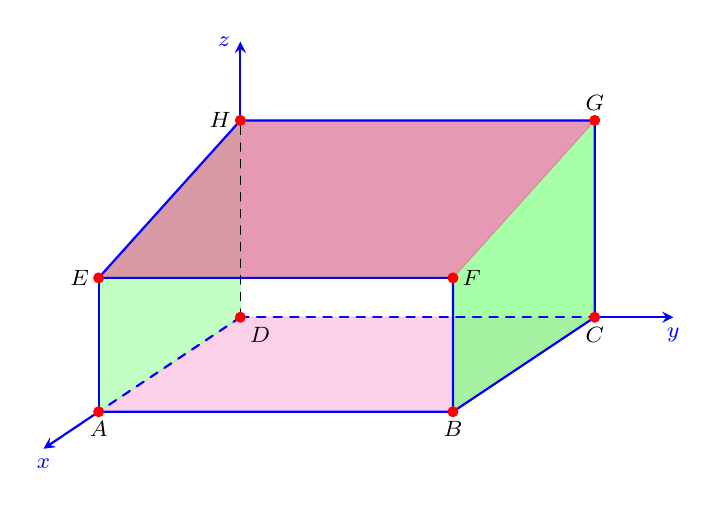
\begin{tikzpicture}[scale=1, font=\footnotesize, line join=round, line cap=round, >=stealth]
	\coordinate (D) at (0,0);
	\coordinate (C) at (4.5,0);
	\coordinate (H) at (0,2.5);
	\coordinate (G) at (4.5,2.5);
	\coordinate (A) at (-1.8,-1.2);
	\coordinate (B) at (2.7,-1.2);
	\coordinate (E) at (-1.8,0.5);
	\coordinate (F) at (2.7,0.5);
	\draw[fill,magenta!30, opacity=0.6] (A) -- (B) -- (C) -- (D) -- cycle;
	\draw[fill,green!40, opacity=0.6] (A) -- (E) -- (H) -- (D) -- cycle;
	\draw[fill,green!50, opacity=0.7] (B) -- (F) -- (G) -- (C) -- cycle;
	\draw[fill,purple!50, opacity=0.8] (E) -- (F) -- (G) -- (H) -- cycle;
	\draw[->,thick, blue] (H) -- (0,3.5) node[left] {$z$};
	\draw[->,thick, blue] (C) -- (5.5,0) node[below] {$y$};
	\draw[->,thick, blue] (A) -- (-2.5,-1.67) node[below] {$x$};
	\draw[dashed] (D) -- (H);
	\draw[thick, blue, dashed] (D) -- (C);
	\draw[thick, blue, dashed] (D) -- (A);
	\draw[thick, blue] (A) -- (B)--(C)--(G)--(H)--(E)--(F)--(B);
	\draw[thick, blue] (E) -- (A);
	\foreach \p in {A,B,C,D,E,F,G,H}
	\fill[red] (\p) circle (2pt);
	\node[below] at (A) {$A$};
	\node[below] at (B) {$B$};
	\node[below] at (C) {$C$};
	\node[below right] at (D) {$D$};
	\node[left] at (E) {$E$};
	\node[right] at (F) {$F$};
	\node[above] at (G) {$G$};
	\node[left] at (H) {$H$};
	\end{tikzpicture}
	\end{center}
	\choiceTF
	{\True Điểm $A\left(6;0;0\right)$}
	{Phương trình mặt phẳng $(EFGH)$ có dạng $ax+by+cz-150=0$. Khi đó $a+b+c=23$}
	{\True Giá một $m^2$ lưới chống nắng là $12\,000$ đồng. Khi đó, số tiền ông Sơn mua lưới lợp mái $EFGH$ là $386$ nghìn đồng (kết quả làm tròn đến hàng nghìn đồng)}
	{\True Ông Sơn cần lắp đặt dây từ điểm $I$ nằm trên cạnh $AB$ và cách $B$ một mét, đến điểm $M$ nằm trên cạnh $BC$, đến điểm $N$ nằm trên cạnh $CG$, đến điểm $P$ nằm trên cạnh $DH$ và đến điểm $E$. Biết dây luôn áp sát vào các mặt, độ dài ngắn nhất của dây là $\sqrt{305}$ ($m$)}
	\loigiai{
	\begin{itemchoice}
	\itemch Dựa vào hệ trục tọa độ $Oxyz$ với $D$ trùng với gốc tọa độ $O\left(0;0;0\right)$, chiều dài $AD = 6$ nằm trên trục $Ox$ nên tọa độ điểm $A$ là $\left(6;0;0\right)$.
	\itemch Ta có tọa độ các đỉnh của mái che là $H\left(0;0;5\right)$, $G\left(0;5;4\right)$ và $E\left(6;0;3\right)$. \\
	$\vec{HE} = \left(6;0;-2\right)$, $\vec{HG} = \left(0;5;-1\right)$. \\
	Một vectơ pháp tuyến của mặt phẳng $(EFGH)$ là $\vec{n} = \left[\vec{HE}, \vec{HG}\right] = \left(10; 6; 30\right)$. \\
	Phương trình mặt phẳng $(EFGH)$ đi qua $H\left(0;0;5\right)$ là: $10\left(x-0\right) + 6\left(y-0\right) + 30\left(z-5\right) = 0 \Leftrightarrow 10x + 6y + 30z - 150 = 0$. \\
	Khi đó $a=10, b=6, c=30 \Rightarrow a+b+c = 10+6+30 = 46$. 
	\itemch Diện tích mảnh đất $ABCD$ là $S_{ABCD} = 5 \cdot 6 = 30$ ($m^2$). \\
	Gọi $\alpha$ là góc giữa mặt phẳng mái $(EFGH)$ và mặt đất $(ABCD)$. \\
	Vectơ pháp tuyến của $(EFGH)$ là $\vec{n} = \left(10; 6; 30\right)$, của $(ABCD)$ là $\vec{k} = \left(0;0;1\right)$. \\
	Suy ra $\cos \alpha = \dfrac{\left|30\right|}{\sqrt{10^2+6^2+30^2} \cdot 1} = \dfrac{30}{\sqrt{1036}} = \dfrac{30}{2\sqrt{259}} = \dfrac{15}{\sqrt{259}}$. \\
	Diện tích mái $EFGH$ là $S_{EFGH} = \dfrac{S_{ABCD}}{\cos \alpha} = \dfrac{30}{\dfrac{15}{\sqrt{259}}} = 2\sqrt{259} \approx 32{,}187$ ($m^2$). \\
	Số tiền mua lưới là $2\sqrt{259} \cdot 12\,000 \approx 386\,243$ (đồng). \\
	Làm tròn đến hàng nghìn đồng ta được $386$ nghìn đồng. 
	\itemch Hình vẽ sau khi được trải phẳng lên mặt phẳng $(DCGH)$ là
	\begin{center}
	\begin{tikzpicture}[scale=.65, font=\footnotesize, line join=round, line cap=round, >=stealth]
	\draw (0,0) -- (24,0);
	\draw (0,0) -- (0,3); 
	\draw (6,0) -- (6,7); 
	\draw (11,0) -- (11,5.166);
	\draw (24,0) -- (24,-1); 
	\draw[red, thick] (0,3) -- (24,-1);
	\foreach \p in {(0,3), (6,2), (11,1.166), (18,0), (24,-1), (6,0), (11,0), (24,0)}
	\fill[red] \p circle (3pt);
	\node[left] at (0,3) {$E$};
	\node[above] at (6,7) {$H$};
	\node[above] at (11,5.166) {$G$};
	\node[right] at (24,0) {$B$};
	\node[below] at (24,-1) {$I$};
	\node[above right] at (6,2) {$P$};
	\node[above right] at (11,1.166) {$N$};
	\node[above right] at (18,0) {$M$};
	\node[below] at (6,0) {$D$};
	\node[below] at (11,0) {$C$};
	\node[left] at (0,1.5) {$3$};
	\node[below] at (3,0) {$6$};
	\node[left] at (6,4.5) {$5$};
	\node[below] at (8.5,0) {$5$};
	\node[left] at (11,3.166) {$4$};
	\node[below] at (21,0.1) {$6$};
	\node[right] at (24,-0.5) {$1$};
	\end{tikzpicture}
	\begin{tikzpicture}[scale=.8, font=\footnotesize, line join=round, line cap=round, >=stealth]
	\fill[cyan!10] (0,0) rectangle (6,5);
	\fill[green!10] (0,5) -- (6,5) -- (6,8) -- (0,9) -- cycle;
	\fill[orange!10] (6,5) -- (11,5) -- (11,9) -- (6,8) -- cycle;
	\fill[violet!10] (11,5) -- (17,5) -- (17,8) -- (11,9) -- cycle;
	\draw (0,0) -- (6,0) -- (6,5) -- (0,5) -- cycle;
	\draw (0,5) -- (0,9) -- (6,8) -- (6,5);
	\draw (6,8) -- (11,9) -- (11,5) -- (6,5);
	\draw (11,9) -- (17,8) -- (17,5) -- (11,5);
	\node at (3,2.5) {Mặt đáy $ABCD$};
	\node at (3,6.5) {\footnotesize Mặt bên $BCFG$};
	\node at (8.5,6.7) {\footnotesize Mặt sau $CDHG$};
	\node at (14,6.5) {\footnotesize Mặt bên trái $DAEH$};
	\fill (0,0) circle (2pt) node[left] {$A$};
	\fill (0,5) circle (2pt) node[left] {$B$};
	\fill (6,5) circle (2pt) node[below right] {$C$};
	\fill (6,0) circle (2pt) node[above right] {$D$};
	\fill (6,8) circle (2pt) node[above] {$G$};
	\fill (11,9) circle (2pt) node[above] {$H$};
	\fill (17,8) circle (2pt) node[above right] {$E$};
	\coordinate (I) at (0,4.2);
	\coordinate (M) at (4.4,5);
	\coordinate (N) at (6,5.35);
	\coordinate (P) at (11,6.5);
	\coordinate (E) at (17,8);
	\fill (I) circle (2pt) node[left] {$I$};
	\fill (M) circle (2pt) node[above] {$M$};
	\fill (N) circle (2pt) node[above right] {$N$};
	\fill (P) circle (2pt) node[above right] {$P$};
	\draw[red, thick] (I) -- (M) -- (N) -- (P) -- (E);
	\draw[<->] (-0.5,0) -- (-0.5,5) node[midway, left] {$5$};
	\draw[<->] (0,-0.6) -- (6,-0.6) node[midway, below] {$6$};
	\draw[<->] (6,4.4) -- (11,4.4) node[midway, below] {$5$};
	\draw[<->] (11,4.4) -- (17,4.4) node[midway, below] {$6$};
	\draw[<->] (17.5,5) -- (17.5,8) node[midway, right] {$3$};
	\draw[<->] (3,9.1) -- (6,9.1) node[midway, above] {$4$};
	\draw[<->] (11,9.6) -- (17,9.6) node[midway, above] {$5$};
	\end{tikzpicture}
	\end{center}
	Ông Sơn cần lắp đặt dây từ điểm $I$ nằm trên cạnh $AB$ và cách $B$ một mét, đến điểm $M$ nằm trên cạnh $BC$, đến điểm $N$ nằm trên cạnh $CG$, đến điểm $P$ nằm trên cạnh $DH$, và đến điểm $E$ sao cho dây luôn áp sát vào các mặt, độ dài dây ngắn nhất khi $I, M, N, P, E$ thẳng hàng. Độ dài ngắn nhất của dây là $\sqrt{17^2 + 4^2} = \sqrt{305}\, (m)$.
	\end{itemchoice}	
	}
\end{ex}
%%---Câu 4---%%
\begin{ex}%[0D0V2-5]
	Trong một bài kiểm tra trắc nghiệm có $50$ câu hỏi, mỗi câu có bốn phương án trả lời $A$, $B$, $C$, $D$ trong đó chỉ có một phương án trả lời đúng. Mỗi câu trả lời đúng được cộng $0{,}2$ điểm và mỗi câu trả lời sai bị trừ $0,1$ điểm. Trong $50$ câu trên, bạn Nam đã làm được và chắc đúng $35$ câu, $15$ câu còn lại bạn không biết làm nên ở mỗi câu bạn chọn ngẫu nhiên một đáp án.
	\choiceTF
	{\True Ở mỗi câu còn lại, xác suất để bạn Nam làm đúng là $\dfrac{1}{4}$}
	{\True Nếu trong $15$ câu còn lại bạn Nam tô ngẫu nhiên và đúng thêm $3$ câu nữa, khi đó bài của bạn Nam được $6{,}4$ điểm}
	{Bạn Nam làm được $7,0$ điểm, khi đó bạn Nam làm đúng $35$ câu và sai $15$ câu}
	{\True Xác suất để bạn Nam đạt được $7{,}0$ điểm là $0{,}165$ (kết quả làm tròn đến hàng phần nghìn)}
	\loigiai{
	\begin{itemchoice}
	\itemch Trong một câu có bốn phương án trả lời, có đúng một phương án đúng.\\
	Suy ra xác suất để bạn Nam làm đúng ở mỗi câu còn lại là $\dfrac{1}{4}$.
	\itemch Như vậy bài của bạn Nam đúng được $38$ câu và sai $12$ câu.\\
	Do đó số điểm của bài bạn Nam là: $38 \times 0{,}2 - 12 \times 0{,}1 = 6{,}4$.
	\itemch Gọi $x$ là số câu đúng Nam chọn được để bạn Nam được $7{,}0$ điểm.\\
	Ta có $0{,}2x - \left(50 - x\right) \cdot 0{,}1 = 7 \Leftrightarrow 0{,}3x = 12 \Leftrightarrow x = 40$.\\
	Như vậy để được $7,0$ điểm bạn Nam phải làm đúng $40$ câu.
	\itemch Gọi $x$ là số câu đúng Nam chọn được để bạn Nam được $7{,}0$ điểm.\\
	Ta có $0{,}2x - \left(50 - x\right) \cdot 0{,}1 = 7 \Leftrightarrow x = 40$.\\
	Vì bạn Nam đã chắc chắn đúng $35$ câu nên để được $7,0$ điểm bạn Nam cần trả lời đúng thêm $5$ câu trong $15$ câu chọn ngẫu nhiên còn lại.\\
	Vậy xác suất Nam đạt $7{,}0$ điểm môn Toán trong kì thi trên là $p = \mathrm{C}_{15}^5 \cdot \left(\dfrac{1}{4}\right)^5 \cdot \left(\dfrac{3}{4}\right)^{10} \approx 0{,}165$.
	\end{itemchoice}
	}
\end{ex}
\Closesolutionfile{ans}
\caukq
\Opensolutionfile{ans}[ans/02-26-2-ThanhHoa-SoGD-L1-P3]
%%---Câu 1---%%
\begin{ex}%[1H8V5-4]
	Cho hình chóp $S.ABC$ có đáy là tam giác đều cạnh bằng $6$. Hình chiếu vuông góc của đỉnh $S$ trên mặt phẳng $\left( ABC \right)$ là điểm $H$ thuộc cạnh $AB$ sao cho $HA = 2HB$. Góc giữa đường thẳng $SC$ và mặt phẳng $\left( ABC \right)$ bằng $60^\circ$. Tính khoảng cách giữa hai đường thẳng $SA$ và $BC$ (làm tròn đến hàng phần trăm).
	\shortans{$4{,}86$}
	\loigiai{
	\begin{center}
	\begin{tikzpicture}[scale=1.4, font=\footnotesize, line join=round, line cap=round]
	\coordinate (A) at (0,0);
	\coordinate (B) at (5,0);
	\coordinate (C) at (1.2,-2);
	\coordinate (M) at (2.5,0);
	\coordinate (H) at ($(A)!0.72!(B)$);
	\coordinate (S) at ($(H)+(0,3.8)$);
	\coordinate (N) at ($(C)!0.55!(B)$);
	\coordinate (K) at ($(C)!0.78!(B)$);
	\coordinate (I) at ($(A)!0.62!(S)$);
	\coordinate (E) at (1.5,0.8); 
	\draw[dashed] (S)--(H);
	\draw[dashed] (H)--(A) (H)--(C) (H)--(M) (H)--(K);
	\draw[dashed] (A)--(N) (A)--(E) (H)--(E) (H)--(I);
	\draw (S)--(A); 
	\draw (S)--(C); 
	\draw (S)--(B) (A)--(C) (C)--(B);
	\path pic[angle radius=3mm,draw] {right angle = A--E--H};
	\path pic[angle radius=3mm,draw] {right angle = S--H--B};
	\path pic[angle radius=3mm,draw] {right angle = S--H--C};
	\path pic[angle radius=3mm,draw] {right angle = H--K--C};
	\path pic[angle radius=3mm,draw,angle eccentricity=1.5] {angle = H--C--S};
	\path pic[angle radius=3mm,draw] {right angle = A--N--C};
	\path pic[angle radius=3mm,draw] {right angle = A--I--H};
	\node at (1.65,-1.48) {$60^\circ$};
	\foreach \p in {A, B, C, S, H, M, N, E, I, K} {
	\fill (\p) circle (1.2pt);
	}
	\draw[dashed] (H)--(B);
	\node[left] at (A) {$A$};
	\node[right] at (B) {$B$};
	\node[below left] at (C) {$C$};
	\node[above] at (S) {$S$};
	\node[below right] at (H) {$H$};
	\node[below, xshift=-2pt] at (M) {$M$};
	\node[below] at (N) {$N$};
	\node[below right] at (K) {$K$};
	\node[above left] at (E) {$E$};
	\node[left, xshift=-2pt] at (I) {$I$};
	\end{tikzpicture}
	\end{center}
	Gọi $N$ là trung điểm $BC$. Trong mặt phẳng $\left( ABC \right)$ dựng đường thẳng $d$ qua $A$ và song song với $BC$. Qua $H$ dựng đường thẳng song song với $AN$ cắt $d$ tại $E$ và cắt $BC$ tại $K$. Khi đó tứ giác $AEKN$ là hình chữ nhật.\\
	Ta có: $BC \parallel AE \Rightarrow BC \parallel \left( SAE \right) \Rightarrow \mathrm{d}\left( BC, SA \right) = \mathrm{d}\left( BC, \left( SAE \right) \right) = \mathrm{d}\left( K, \left( SAE \right) \right)$.\\
	Mặt khác $\dfrac{HB}{HA} = \dfrac{HK}{HE} = \dfrac{1}{2} \Rightarrow \dfrac{KH}{KE} = \dfrac{1}{3} \Rightarrow \mathrm{d}\left( K, \left( SAE \right) \right) = \dfrac{3}{2} \mathrm{d}\left( H, \left( SAE \right) \right)$.\\
	Ta có $\heva{& AE \perp SH \\& AE \perp KE } \Rightarrow AE \perp \left( SHE \right) \Rightarrow \left( SHE \right) \perp \left( SAE \right)$.\\
	Trong mặt phẳng $\left( SHE \right)$ kẻ $HI \perp SE$ tại $I$. Từ đó suy ra:\\
	$HI \perp \left( SAE \right) \Rightarrow \mathrm{d}\left( H, \left( SAE \right) \right) = HI \Rightarrow d\left( BC, SA \right) = \dfrac{3}{2} HI$.\\
	$HK = \dfrac{1}{3} AN \Rightarrow EH = \dfrac{2}{3} AN = 2\sqrt{3} \Rightarrow HI = \dfrac{SH \cdot HE}{\sqrt{S H^{2} + H E^{2}}} = \dfrac{\sqrt{42}}{2}$.\\
	Vậy $\mathrm{d}\left( SA, BC \right) = \dfrac{3\sqrt{42}}{4} \approx 4{,}86$.
	}
\end{ex}
%%---Câu 2---%%
\begin{ex}%[2D1V3-6]
	Nếu một doanh nghiệp sản xuất $x$ sản phẩm trong một tháng ($x \in \mathbb{N}$; $1 \le x \le 300$) thì doanh thu nhận được khi bán hết số sản phẩm là $F(x) = x^3 - 1\,999x^2 + 1\,001\,000x + 250\,000$ (đồng). Trong đó, chi phí vận hành máy móc bình quân cho mỗi sản phẩm khi sản xuất $x$ sản phẩm là $G(x) = 300 + \dfrac{100}{x}$ (nghìn đồng), chi phí mua nguyên vật liệu để sản xuất $x$ sản phẩm là $H(x) = 2x^3 + 100\,000x - 50\,000$ (đồng). Doanh nghiệp cần sản xuất bao nhiêu sản phẩm để lợi nhuận thu được là lớn nhất?
	\shortans{$136$}
	\loigiai{
	Ta có lợi nhuận được tính như sau:\\
	$\begin{aligned}[t]
	L(x) &= x^3 - 1\,999x^2 + 1\,001\,000x + 250\,000 - x \cdot \left( 300 + \frac{100}{x} \right) \cdot 1\,000 - \left( 2x^3 + 100\,000x - 50\,000 \right)\\
	&= -x^3 - 1\,999x^2 + 601\,000x + 200\,000.	\end{aligned}$\\
	$\Rightarrow L'(x) = 0 \Leftrightarrow x \approx 136{,}37\in [1;300]$.\\
	Bảng biến thiên
	\begin{center}
		
\begin{tikzpicture}[>=stealth]
			\tkzTabInit[nocadre=false,lgt=1.2,espcl=3,deltacl=1.25]
			{$x$/.6 ,$L'(x)$/.6,$y$/2}
			{$1$ , $136{,}37$ , $300$}
			\tkzTabLine{ , + , $0$ , - , }
			\tkzTabVar{-/$799\,000$ , +/$42\,447\,371$ , -/$-26\,410\,000$}
		\end{tikzpicture}
	\end{center}
	Vì số sản phẩm sản xuất được là số tự nhiên, từ bảng biến thiên ta so sánh $L(136)$ và $L(137)$.\\
	Ta có: $L(136) = 42\,447\,040$ ($\text{đồng}$) và $L(137) = 42\,446\,416$ (đồng).\\
	Vậy doanh nghiệp cần sản xuất $136$ sản phẩm thì lợi nhuận là lớn nhất.
	}
\end{ex}
%%---Câu 3---%%
\begin{ex}%[2D4T3-7]
	Một vật bắt đầu chuyển động thẳng đều với vận tốc $v_0 = a$ ($m/s$) với $a > 0$. Sau $6$ giây chuyển động thì gặp chướng ngại vật nên bắt đầu giảm tốc độ với vận tốc chuyển động $v(t) = -\dfrac{5}{2}t + b$ ($m/s$), ($t \ge 6$) cho đến khi dừng hẳn. Biết rằng, kể từ lúc chuyển động đến lúc dừng thì vật đi được quãng đường là $80$ ($m$). Giá trị của $a^2 - b^2$ bằng bao nhiêu?
	\shortans{$-525$}
	\loigiai{
	Tại thời điểm $t = 6$ vật đang chuyển động với vận tốc $v_0 = a$ nên có $v(6) = a$\\
	$\Leftrightarrow -\dfrac{5}{2} \cdot 6 + b = a \Leftrightarrow b = a + 15$, suy ra $v(t) = -\dfrac{5}{2}t + a + 15$.\\
	Gọi $k$ là thời điểm vật dừng hẳn, vậy ta có $v(k) = 0 \Leftrightarrow k = \dfrac{2}{5} \cdot \left( a + 15 \right) \Leftrightarrow k = \dfrac{2a}{5} + 6$.\\
	Tổng quãng đường vật đi được là $80 = 6 \cdot a + \displaystyle\int\limits_{6}^{k} \left( -\dfrac{5}{2}t + a + 15 \right) \text{d}t$\\
	$\Leftrightarrow 80 = 6a + \left. \left( -\dfrac{5}{4}t^2 + at + 15t \right) \right|_{6}^{k}$\\
	$\Leftrightarrow 80 = 6a - \dfrac{5}{4} \cdot \left( k^2 - 6^2 \right) + a \cdot \left( k - 6 \right) + 15 \cdot \left( k - 6 \right)$\\
	$\Leftrightarrow a^2 + 30a - 400 = 0$\\
	$\Leftrightarrow a = 10$ (do $a > 0$).\\
	Với $a = 10 \Rightarrow b = 25$.\\
	Khi đó $a^2 - b^2 = 10^2 - 25^2 = -525$.
	}
\end{ex}
%%---Câu 4---%%
\begin{ex}%[0D0C2-7]
	Lấy ngẫu nhiên một số tự nhiên có $5$ chữ số. Xác suất để chọn được số tự nhiên có dạng $\overline{a_1a_2a_3a_4a_5}$, trong đó $a_1 \le a_2+1 \le a_3-7 < a_4 \le a_5+2$ bằng $a$. Giá trị của $\dfrac{1}{a}$ bằng bao nhiêu (làm tròn đến hàng đơn vị)?
	\shortans{$506$}
	\loigiai{
	Số các số tự nhiên có năm chữ số được lập là $90\,000$ số. \\
	Do $a_2 + 1 \le a_3 - 7 \Rightarrow a_3 \ge a_2 + 8 \Rightarrow \heva{&a_2 \le 1 \\& a_3 \ge 8.}$\\
	\textbf{TH1:} Nếu $a_2 = 0$, $a_1 = 1$ và $a_3 = 8$. \\
	Khi đó $a_4 > 8 - 7 = 1$ nên $a_4 \in \{2, 3, \dots, 9\}$. \\
	Với $a_4 = 2$ thì $a_5 + 2 \ge 2 \Rightarrow a_5 \ge 0$ nên $a_5$ có $10$ cách chọn. \\
	Với $a_4 = 3$ thì $a_5 + 2 \ge 3 \Rightarrow a_5 \ge 1$ nên $a_5$ có $9$ cách chọn. \\
	\ldots \\
	Với $a_4 = 9$ thì $a_5 + 2 \ge 9 \Rightarrow a_5 \ge 7$ nên $a_5$ có $3$ cách chọn. \\
	Do đó số các số được lập trong trường hợp này là: $10 + 9 + \dots + 3 = 52$. \\
	\textbf{TH2:} Nếu $a_2 = 0$, $a_1 = 1$ và $a_3 = 9$. \\
	Khi đó $a_4 > 9 - 7 = 2$ nên $a_4 \in \{3, 4, \dots, 9\}$. \\
	Với $a_4 = 3$ thì $a_5 + 2 \ge 3 \Rightarrow a_5 \ge 1$ nên $a_5$ có $9$ cách chọn. \\
	Với $a_4 = 4$ thì $a_5 + 2 \ge 4 \Rightarrow a_5 \ge 2$ nên $a_5$ có $8$ cách chọn. \\
	\ldots\\
	Với $a_4 = 9$ thì $a_5 + 2 \ge 9 \Rightarrow a_5 \ge 7$ nên $a_5$ có $3$ cách chọn. \\
	Do đó số các số được lập trong trường hợp này là: $9 + 8 + \dots + 3 = 42$ số. \\
	\textbf{TH3:} Nếu $a_2 = 1$, thì $a_1 \le a_2 + 1 = 2$ nên $a_1$ có $2$ cách chọn ($a_1 \in \{1, 2\}$). \\
	Với mỗi cách chọn của $a_1$, ta có $a_3 \ge a_2 + 8 = 9 \Rightarrow a_3 = 9$. \\
	Khi đó $a_4 > 9 - 7 = 2$ nên: \\
	Với $a_4 = 3$ thì $a_5 \ge 1$ nên $a_5$ có $9$ cách chọn. \\
	Với $a_4 = 4$ thì $a_5 \ge 2$ nên $a_5$ có $8$ cách chọn. \\
	\ldots \\
	Với $a_4 = 9$ thì $a_5 \ge 7$ nên $a_5$ có $3$ cách chọn. \\
	Do đó số các số được lập trong trường hợp này là: $2 \times \left(9 + 8 + \dots + 3\right) = 2 \times 42 = 84$ số. \\
	Do đó tổng số các số thỏa mãn bài ra là: $52 + 42 + 84 = 178$ số. \\
	Suy ra xác suất cần tính bằng $a = \dfrac{178}{90\,000} = \dfrac{89}{45\,000} \Rightarrow \dfrac{1}{a} = \dfrac{45\,000}{89} \approx 505{,}617$. \\
	Làm tròn đến hàng đơn vị, ta được giá trị $\dfrac{1}{a} \approx 506$.
	}
\end{ex}
%%---Câu 5---%%
\begin{ex}%[2H5C1-7]
	Trong không gian $Oxyz$, cho ba điểm $A\left(-1; -4; 4\right)$, $B\left(-1; -2; 4\right)$ và $C\left(0; -4; 4\right)$. Mặt phẳng $(P)$ có dạng $ax + 2\,025y + cz + d = 0$ đi qua điểm $A$ sao cho hai điểm $B, C$ nằm về cùng một phía. Đặt $h_1 = d\left(B, (P)\right)$ là khoảng cách từ điểm $B$ đến mặt phẳng $(P)$ và $h_2 = d\left(C, (P)\right)$ là khoảng cách từ điểm $C$ đến mặt phẳng $(P)$. Khi biểu thức $2\,025h_1 + 2\,026h_2$ đạt giá trị lớn nhất, giá trị của biểu thức $T = -9a + 10c + d$ bằng bao nhiêu?
	\shortans{$-4$}
	\loigiai{
	\begin{center}
	\begin{tikzpicture}[scale=1.4, font=\footnotesize, line join=round, line cap=round]
	\coordinate (H) at (0,0);
	\coordinate (M) at (0,3);
	\coordinate (K) at (7,0.5);
	\coordinate (A) at (3,-1.0);
	\coordinate (N) at (7,5);
	\coordinate (I) at ($(M)!0.5!(N)$);
	\coordinate (J) at ($(H)!0.5!(K)$);
	\coordinate (B) at ($(M)!0.6!(A)$);
	\coordinate (C) at ($(N)!0.65!(A)$);
	\coordinate (E) at ($(H)!0.6!(A)$);
	\coordinate (F) at ($(K)!0.65!(A)$);
	\foreach \p in {A, B, C, K, H, M, N,I} {
	\fill (\p) circle (1.2pt);
	}
	\draw[dashed] (H)--(K);
	\draw[dashed] (I)--(J);
	\draw (M)--(A) (N)--(A) (B)--(C) (B)--(E) (C)--(F);
	\draw (M)--(H) (H)--(A) (K)--(A) (M)--(N) (K)--(N);
	\node[left] at (H) {$H$};
	\node[right] at (K) {$K$};
	\node[below left] at (A) {$A$};
	\node[above] at (M) {$M$};
	\node[right] at (N) {$N$};
	\node[above] at (I) {$I$};
	\node[below right] at (C) {$C$};
	\node[above right] at (B) {$B$};
	\path (I)--(J)node[pos=0.5,black,left]{$d$};
	\path (B)--(E)node[pos=0.5,black,left]{$h_1$};
	\path (C)--(F)node[pos=0.3,black,right]{$h_2$};
	\path pic[angle radius=3mm,draw] {right angle = B--E--A};
	\path pic[angle radius=3mm,draw] {right angle = C--F--A};
	\end{tikzpicture}
	\end{center}
	Gọi $M$ là điểm thỏa mãn $\overrightarrow{AM} = 2\,025 \cdot \overrightarrow{AB}$, suy ra $M\left(-1; 4\,046; 4\right)$.\\
	Khi đó $2\,025h_1 = 2\,025 \cdot \mathrm{d}\left(B, (P)\right) = \mathrm{d}\left(M, (P)\right)$.\\
	Gọi $N$ là điểm thỏa mãn $\overrightarrow{AN} = 2\,026 \cdot \overrightarrow{AC}$, suy ra $N\left(2\,025; -4; 4\right)$.\\
	Khi đó $2\,026h_2 = 2\,026 \cdot \mathrm{d}\left(C, (P)\right) = \mathrm{d}\left(N, (P)\right)$.\\
	Suy ra $2\,025h_1 + 2\,026h_2 = \mathrm{d}\left(M, (P)\right) + \mathrm{d}\left(N, (P)\right)$.\\
	Gọi $I$ là trung điểm của $MN$, suy ra $I\left(1\,012; 2\,021; 4\right)$.\\
	Khi đó $2\,025h_1 + 2\,026h_2 = \mathrm{d}\left(M, (P)\right) + \mathrm{d}\left(N, (P)\right) = 2\mathrm{d}\left(I, (P)\right) \le 2IA$.\\
	Do vậy $2\,025h_1 + 2\,026h_2$ đạt giá trị lớn nhất khi $(P)$ qua $A$ và vuông góc với $IA$.\\
	Hay $(P)$ đi qua $A\left(-1; -4; 4\right)$ và nhận $\overrightarrow{AI} = \left(1\,013; 2\,025; 0\right)$ làm vectơ pháp tuyến.\\
	Phương trình mặt phẳng $(P): 1\,013x + 2\,025y + 9\,113 = 0$.\\
	Vậy $a = 1\,013$; $c = 0$; $d = 9\,113 \Rightarrow T = -9a + 10c + d = -4$.
	}
\end{ex}
%%---Câu 6---%%
\begin{ex}%[2D4V5-3]
\immini{Một cái chậu đựng nước có dạng hình chóp cụt đều, đáy chậu là tam giác đều cạnh bằng $2\text{ dm}$, miệng chậu là tam giác đều cạnh bằng $5\text{ dm}$ và chiều cao chậu nước bằng $3\text{ dm}$. Người ta bơm nước vào chậu với lưu lượng không đổi $\dfrac{\sqrt{3}}{3}$ lít/phút. Tại thời điểm $14$ phút sau khi bơm tốc độ dâng lên của nước trong chậu là $\dfrac{1}{a} \text{ dm/phút}$, giá trị của $a$ bằng bao nhiêu?
}{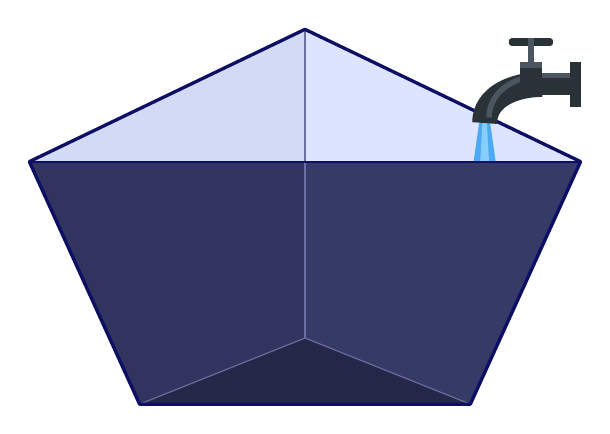
\begin{tikzpicture}[scale=1.4]
	% Define custom colors
	\definecolor{dryleft}{RGB}{210, 218, 245}
	\definecolor{dryright}{RGB}{220, 228, 255}
	\definecolor{wetleft}{RGB}{48, 52, 94}
	\definecolor{wetright}{RGB}{54, 58, 102}
	\definecolor{wetbottom}{RGB}{36, 40, 72}
	\definecolor{strokecolor}{RGB}{12, 15, 100}
	\definecolor{waterline}{RGB}{80, 100, 180}
	\definecolor{stream}{RGB}{50, 160, 240}
	\definecolor{streamhighlight}{RGB}{140, 210, 255}
	\definecolor{faucet}{RGB}{40, 50, 55}
	\definecolor{faucethigh}{RGB}{75, 85, 95}
	\coordinate (A) at (0, 2.2);     
	\coordinate (B) at (-2.5, 1.0);  
	\coordinate (C) at (2.5, 1.0);   
	\coordinate (D) at (-1.5, -1.2); 
	\coordinate (E) at (1.5, -1.2);  
	\coordinate (F) at (0, -0.6);    
	\coordinate (W) at (0, 1.0);     
	\fill[dryleft] (A) -- (B) -- (W) -- cycle;
	\fill[dryright] (A) -- (C) -- (W) -- cycle;
	\fill[wetleft] (B) -- (W) -- (F) -- (D) -- cycle;
	\fill[wetright] (C) -- (W) -- (F) -- (E) -- cycle;
	\fill[wetbottom] (D) -- (E) -- (F) -- cycle;
	\draw[strokecolor!60, thin] (A) -- (F);
	\draw[strokecolor!60, thin] (D) -- (F);
	\draw[strokecolor!60, thin] (E) -- (F);
	\fill[stream, opacity=0.85] (1.58, 1.35) -- (1.68, 1.35) -- (1.73, 1.0) -- (1.53, 1.0) -- cycle;
	\fill[streamhighlight, opacity=0.9] (1.61, 1.35) -- (1.65, 1.35) -- (1.67, 1.0) -- (1.59, 1.0) -- cycle;
	\draw[strokecolor, very thick, line join=round] (A) -- (B) -- (D) -- (E) -- (C) -- cycle;
	\draw[strokecolor, thick] (B) -- (C);
	\fill[faucet] (2.4, 1.5) rectangle (2.5, 1.9);
	\fill[faucet] (2.1, 1.6) rectangle (2.4, 1.8);
	\fill[faucethigh] (2.1, 1.76) rectangle (2.4, 1.8);
	\draw[faucet, line width=9pt, line cap=butt] (2.15, 1.7) to[out=180, in=90] (1.63, 1.35);
	\draw[faucethigh, line width=2pt, line cap=butt] (2.15, 1.78) to[out=180, in=90] (1.67, 1.4);
	\fill[faucet] (1.95, 1.62) rectangle (2.15, 1.9);
	\fill[faucethigh] (1.95, 1.85) rectangle (2.15, 1.9);
	\fill[faucethigh] (2.02, 1.9) rectangle (2.08, 2.05);
	\fill[faucet, rounded corners=1pt] (1.85, 2.05) rectangle (2.25, 2.12);
	\fill[faucethigh] (2.02, 2.05) rectangle (2.08, 2.12);
\end{tikzpicture}}
	\shortans{$12$}
	\loigiai{
	\begin{center}
	\begin{tikzpicture}[scale=3,>=stealth,line join=round,line cap=round]
	\draw[black] (0,0)coordinate(A)--(0:3)coordinate(B)--($(120:-2)+(0:1)$)coordinate(C)--(120:-2)coordinate(D)--cycle;
	\foreach \diem/\vitrin in {A/left,B/right,C/below,D/left} \fill[black](\diem)circle(1.0pt)node[\vitrin]{$\diem$};
	\coordinate (H) at (1.5,.5);
	\coordinate (J) at (1.5,-1.5);
	\coordinate (K) at (3.5,-1.75);
	\foreach \p in {H,J} {
	\fill (\p) circle (1.0pt);
	}
	\node[above] at (H) {$H$};
	\node[above right] at (J) {$J$};
	\path (A)..controls+(-30:1)and+(150:1)..coordinate[label=left:$M$,pos=0.5](M)(D);
	\path (B)..controls+(-30:1)and+(150:1)..coordinate[label=right:$N$,pos=0.5](N)(C);
	\path (H)..controls+(-30:1)and+(150:1)..coordinate[label=right:$E$,pos=0.5](E)(J);
	\draw (H)--(A) (H)--(B) (M)--(N) ;
	\draw[dashed] (H)--(J) (D)--(J) (C)--(J) (E)--(M) (E)--(N) (C)--(K);
	\path (A)--(H)node[pos=0.5,black,above left]{$5$};
	\path (B)--(H)node[pos=0.5,black,above right]{$5$};
	\path (H)--(E)node[pos=0.5,black,left]{$5$};
	\path (D)--(J)node[pos=0.5,black,above left]{$2$};
	\path (D)--(C)node[pos=0.5,black,below]{$2$};
	\path (C)--(J)node[pos=0.5,black,above right]{$2$};
	\coordinate[] (P) at ($(C)!(B)!(K)$);
	\coordinate[] (Q) at ($(C)!(N)!(K)$);
	\draw[dashed] (N)--(Q) (B)--(P);
	\path (N)--(Q)node[pos=0.5,black,right]{$h$};
	\path (B)--(P)node[pos=0.5,black,right]{$3$};
	\foreach \diem in {E,M,N,P,Q}	\fill (\diem)circle(1.pt);
	\end{tikzpicture}
	\end{center}
	Gọi $MN$ là độ dài cạnh tam giác đều theo mực nước tức thời ($MN$ thay đổi). \\
	Đặt $MN = m \cdot h + n$ (hàm số bậc nhất theo chiều cao mực nước $h$). \\
	Khi $h = 0$ thì $MN = 2$; khi $h = 3$ thì $MN = 5$. \\
	Do đó $\heva{&n = 2 \\& 3m + n = 5} \Rightarrow \heva{&n = 2 \\& m = 1.}$\\
	suy ra $MN = h + 2$. \\
	Diện tích mặt nước tức thời là $S = \dfrac{MN^2 \cdot \sqrt{3}}{4} = \dfrac{(h+2)^2 \cdot \sqrt{3}}{4}$. \\
	Thể tích nước tức thời là $V = \dfrac{1}{3}h \left(S_0 + \sqrt{S_0 S} + S\right)$, với $S_0 = \sqrt{3}$ là diện tích mặt nước ban đầu (đáy nhỏ). \\
	$V = \dfrac{1}{3}h \left( \sqrt{3} + \sqrt{\sqrt{3} \cdot \dfrac{(h+2)^2 \cdot \sqrt{3}}{4}} + \dfrac{(h+2)^2 \cdot \sqrt{3}}{4} \right) = \dfrac{h\sqrt{3}}{12} \left[ 4 + 2(h+2) + (h+2)^2 \right]$. \\
	$V = \dfrac{h\sqrt{3}}{12} \left(h^2 + 6h + 12\right) = \dfrac{\sqrt{3}}{12} \left(h^3 + 6h^2 + 12h\right) \quad (*)$. \\
	Sau $14$ phút thì lượng nước trong chậu là $V = \dfrac{\sqrt{3}}{3} \times 14 = \dfrac{14\sqrt{3}}{3} \text{ dm}^3$ (vì $1$ lít $= 1 \text{ dm}^3$). \\
	Do đó $\dfrac{\sqrt{3}}{12} \left(h^3 + 6h^2 + 12h\right) = \dfrac{14\sqrt{3}}{3} \Rightarrow h^3 + 6h^2 + 12h - 56 = 0 \Rightarrow h = 2 \text{ dm}$. \\
	Từ $(*)$ đạo hàm hai vế theo $t$ ta được: $V'(t) = \dfrac{\sqrt{3}}{12} \left(3h^2 + 12h + 12\right) \cdot h'(t) \quad (**)$. \\
	Thay các giá trị $h = 2$, $V'(t) = \dfrac{\sqrt{3}}{3}$ vào $(**)$ ta được: \\
	$\dfrac{\sqrt{3}}{3} = \dfrac{\sqrt{3}}{12} \left(3 \cdot 2^2 + 12 \cdot 2 + 12\right) \cdot h'(t) \Rightarrow \dfrac{1}{3} = \dfrac{1}{12} \cdot 48 \cdot h'(t) \Rightarrow h'(t) = \dfrac{1}{12} \text{ dm/phút}$. \\
	Theo giả thiết, tốc độ dâng lên của nước là $\dfrac{1}{a} \text{ dm/phút}$, suy ra $a = 12$.
	}
\end{ex}



\Closesolutionfile{ans}